\documentclass{article}

\usepackage[letterpaper, top=1in, bottom=1in, left=1in, right=1in]{geometry}
\usepackage{physics, amsmath, enumitem, nicefrac, fancyhdr, microtype, tikz}

\pagestyle{fancy}

\title{Friction and Circular Motion}
\author{Laith Toom}
\date{21/2/2023}

\begin{document}
\maketitle
\newpage

\section{Friction}
When a object is moving along a surface, there is a force acting 
against that movement, and that force is friction $f$.

\begin{figure}[h]
    \centering
    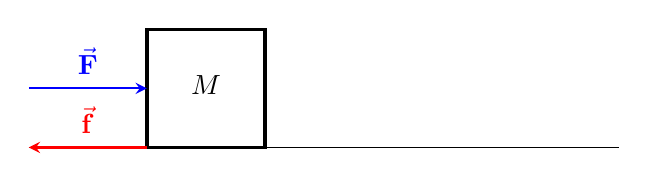
\begin{tikzpicture}[scale=1.5]
        \draw (0, 0) -- (5, 0);

        \draw[very thick] (1, 0) -- (1, 1) -- (2, 1) node[midway, yshift=-20] {$M$} -- (2, 0) --(1, 0);

        \draw[thick, -stealth, blue] (0, 0.5) -- (1, 0.5) node[midway, yshift=10] {$\va{F}$};
        \draw[thick, -stealth, red] (1, 0) -- (0, 0) node[midway, yshift=10] {$\va{f}$};
    \end{tikzpicture}
    \caption{Box moving along ground}
\end{figure}

\newpage
\section{Cricular Motion}


\end{document}